%!TEX root = ../thesis.tex

\section{背景}
% \subsection{RoboCup}
近年,機械学習を用いた自律移動に関しての研究が盛んに行われている.
Bojarskiら\cite{bojarski}は,カメラ画像とステアリングの角度を教師信号とし,end-to-end学習することで自動車の自動運転に成功している.このシステムは,人間からの最小限の学習データで,車線のあるなしを問わず一般道や高速道路での渋滞中の走行を学習する.また,駐車場や未舗装路など,視覚ガイダンスが不明瞭な場所でも運転することができます.本システムは,人間の操舵角のみを学習信号として,道路の特徴を検出するなどの必要な処理を内部表現として自動的に学習させる.このため,例えば,道路の外周を検出するような明示的な学習は行っていない.

\begin{figure}[hbtp]
     \centering
    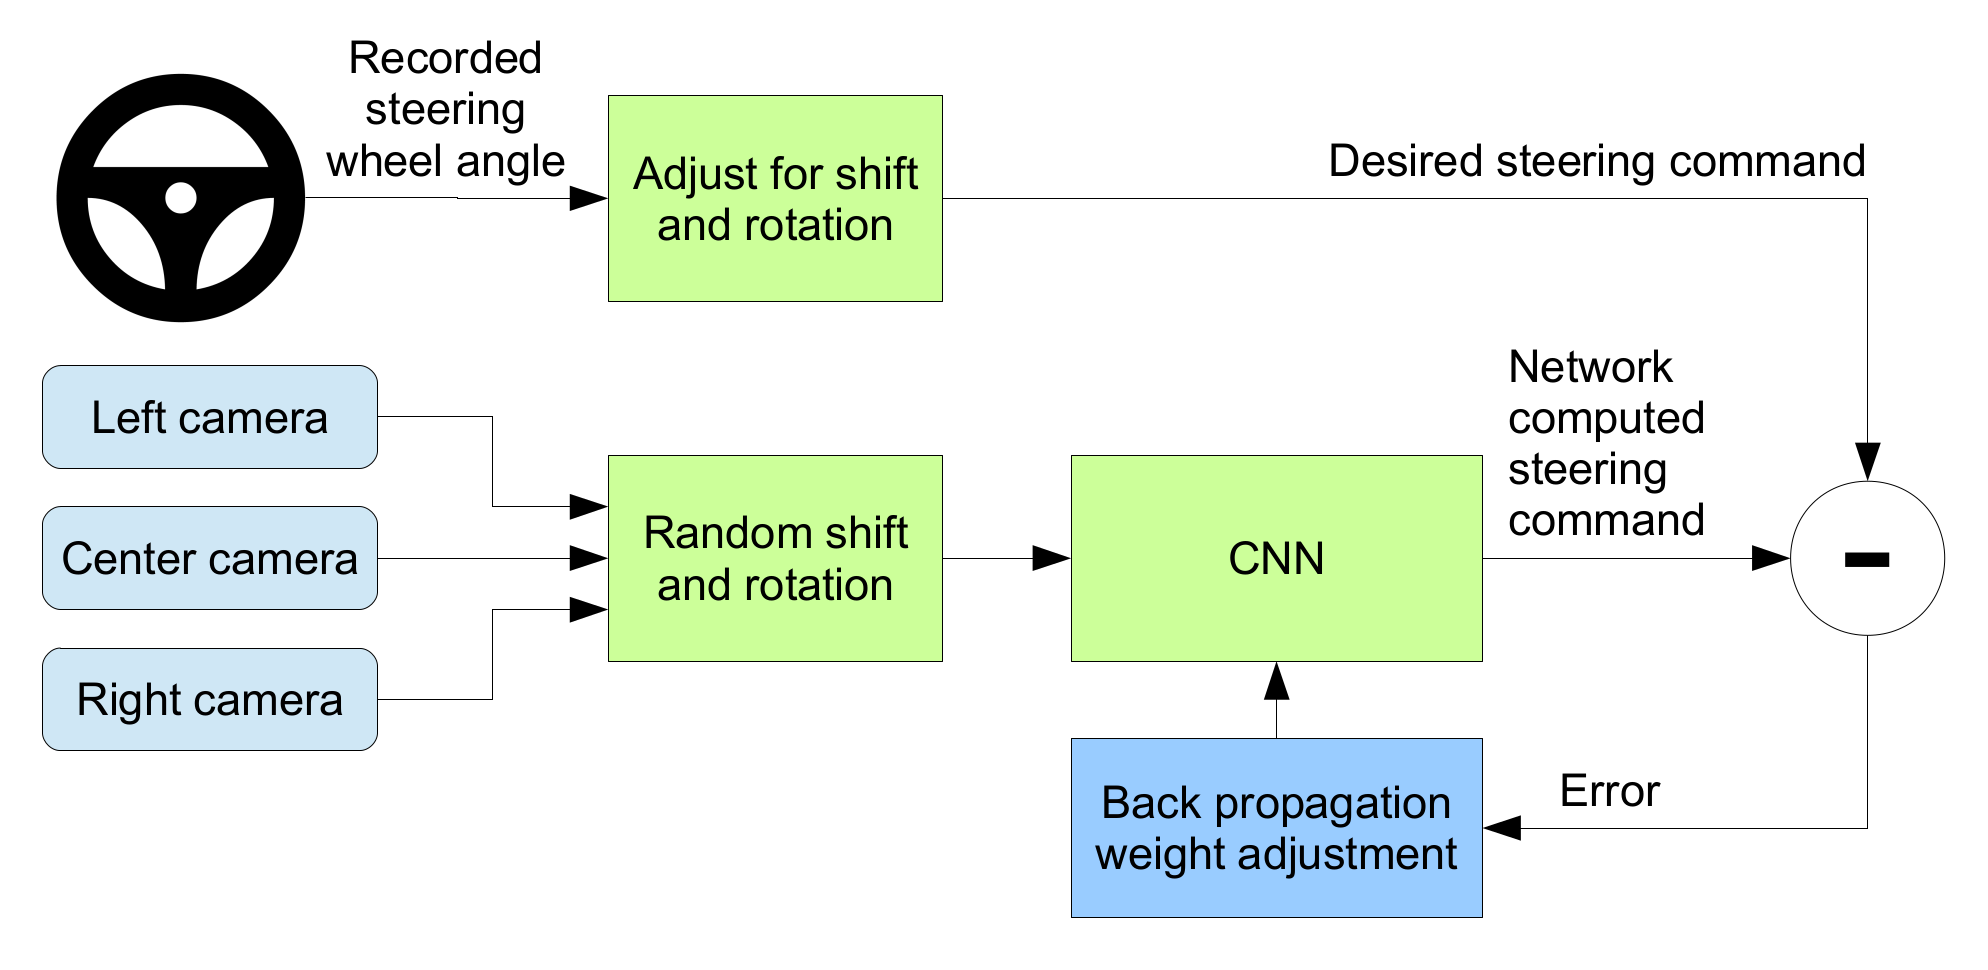
\includegraphics[keepaspectratio, scale=0.16]
         {images/bojarski_train.png}
    \caption{Training the neural network \cite{bojarski}}
    \label{Fig:bojarski_train}
\end{figure}

学習後は,\figref{Fig:bojarski_test}に示すようにカメラ画像から直接ステアリングコマンドを出力するシステムになっている.

\begin{figure}[hbtp]
     \centering
    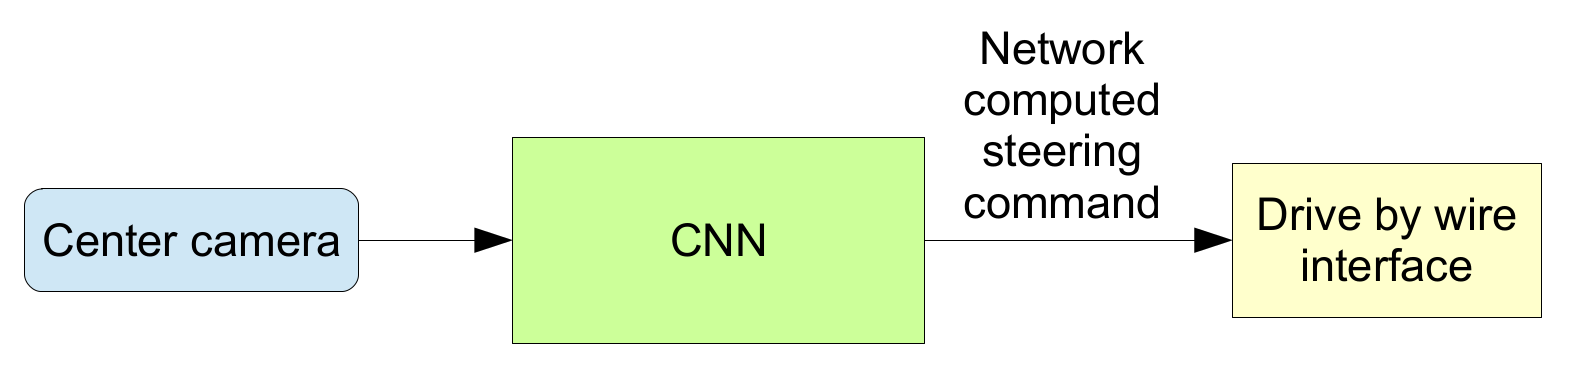
\includegraphics[keepaspectratio, scale=0.16]
         {images/bojarski_test.png}
    \caption{The trained network is used to generate steering commands from a single front-facing center camera. \cite{bojarski}}
    \label{Fig:bojarski_test}
\end{figure}

岡田ら[]はこれらの技術を応用し,カメラ画像に基づく人追従行動を獲得している.ここでの教師信号はカメラ画像とルールベース制御器の出力である.
% \subsubsection{etc...}
\newpage
